This chapter provides background information that will help the reader to understand the research, it introduces general concepts of the wastewater treatment and computational techniques. 

\section{Wastewater Treatment}
\label{s:First-Background-Topic}

\ac{WWT} aims to reduce different contaminants present in water from a diversity of sources. The wastewater pass through several processes to remove the contaminants (mainly nutrients and solids) until the water reaches the standards of quality established by the corresponding regulatory authorities for discharging to a water body or to reuse it. The \ac{WWTP}s are the facilities in charge of this process and involve different stages to achieve their goal. After receiving the raw wastewater, the \ac{WWTP} starts with a physical treatment which comprises the use of screens, grilles and grit traps to remove solids and materials of large size. Then, it is involved the primary treatment to reduce and degrade diverse nutrients and organic compounds, most of the cases it is a Biological or chemical process. After the primary treatment there is a settling or clarifier that allows to separate the already translucent water from some sludge remaining. The cleaner water overflows the clarifier to a final stage of disinfection and pH adjustments to discharge it to the water body minimizing the impact on the ecosystem.

\begin{figure}[h]
\centering
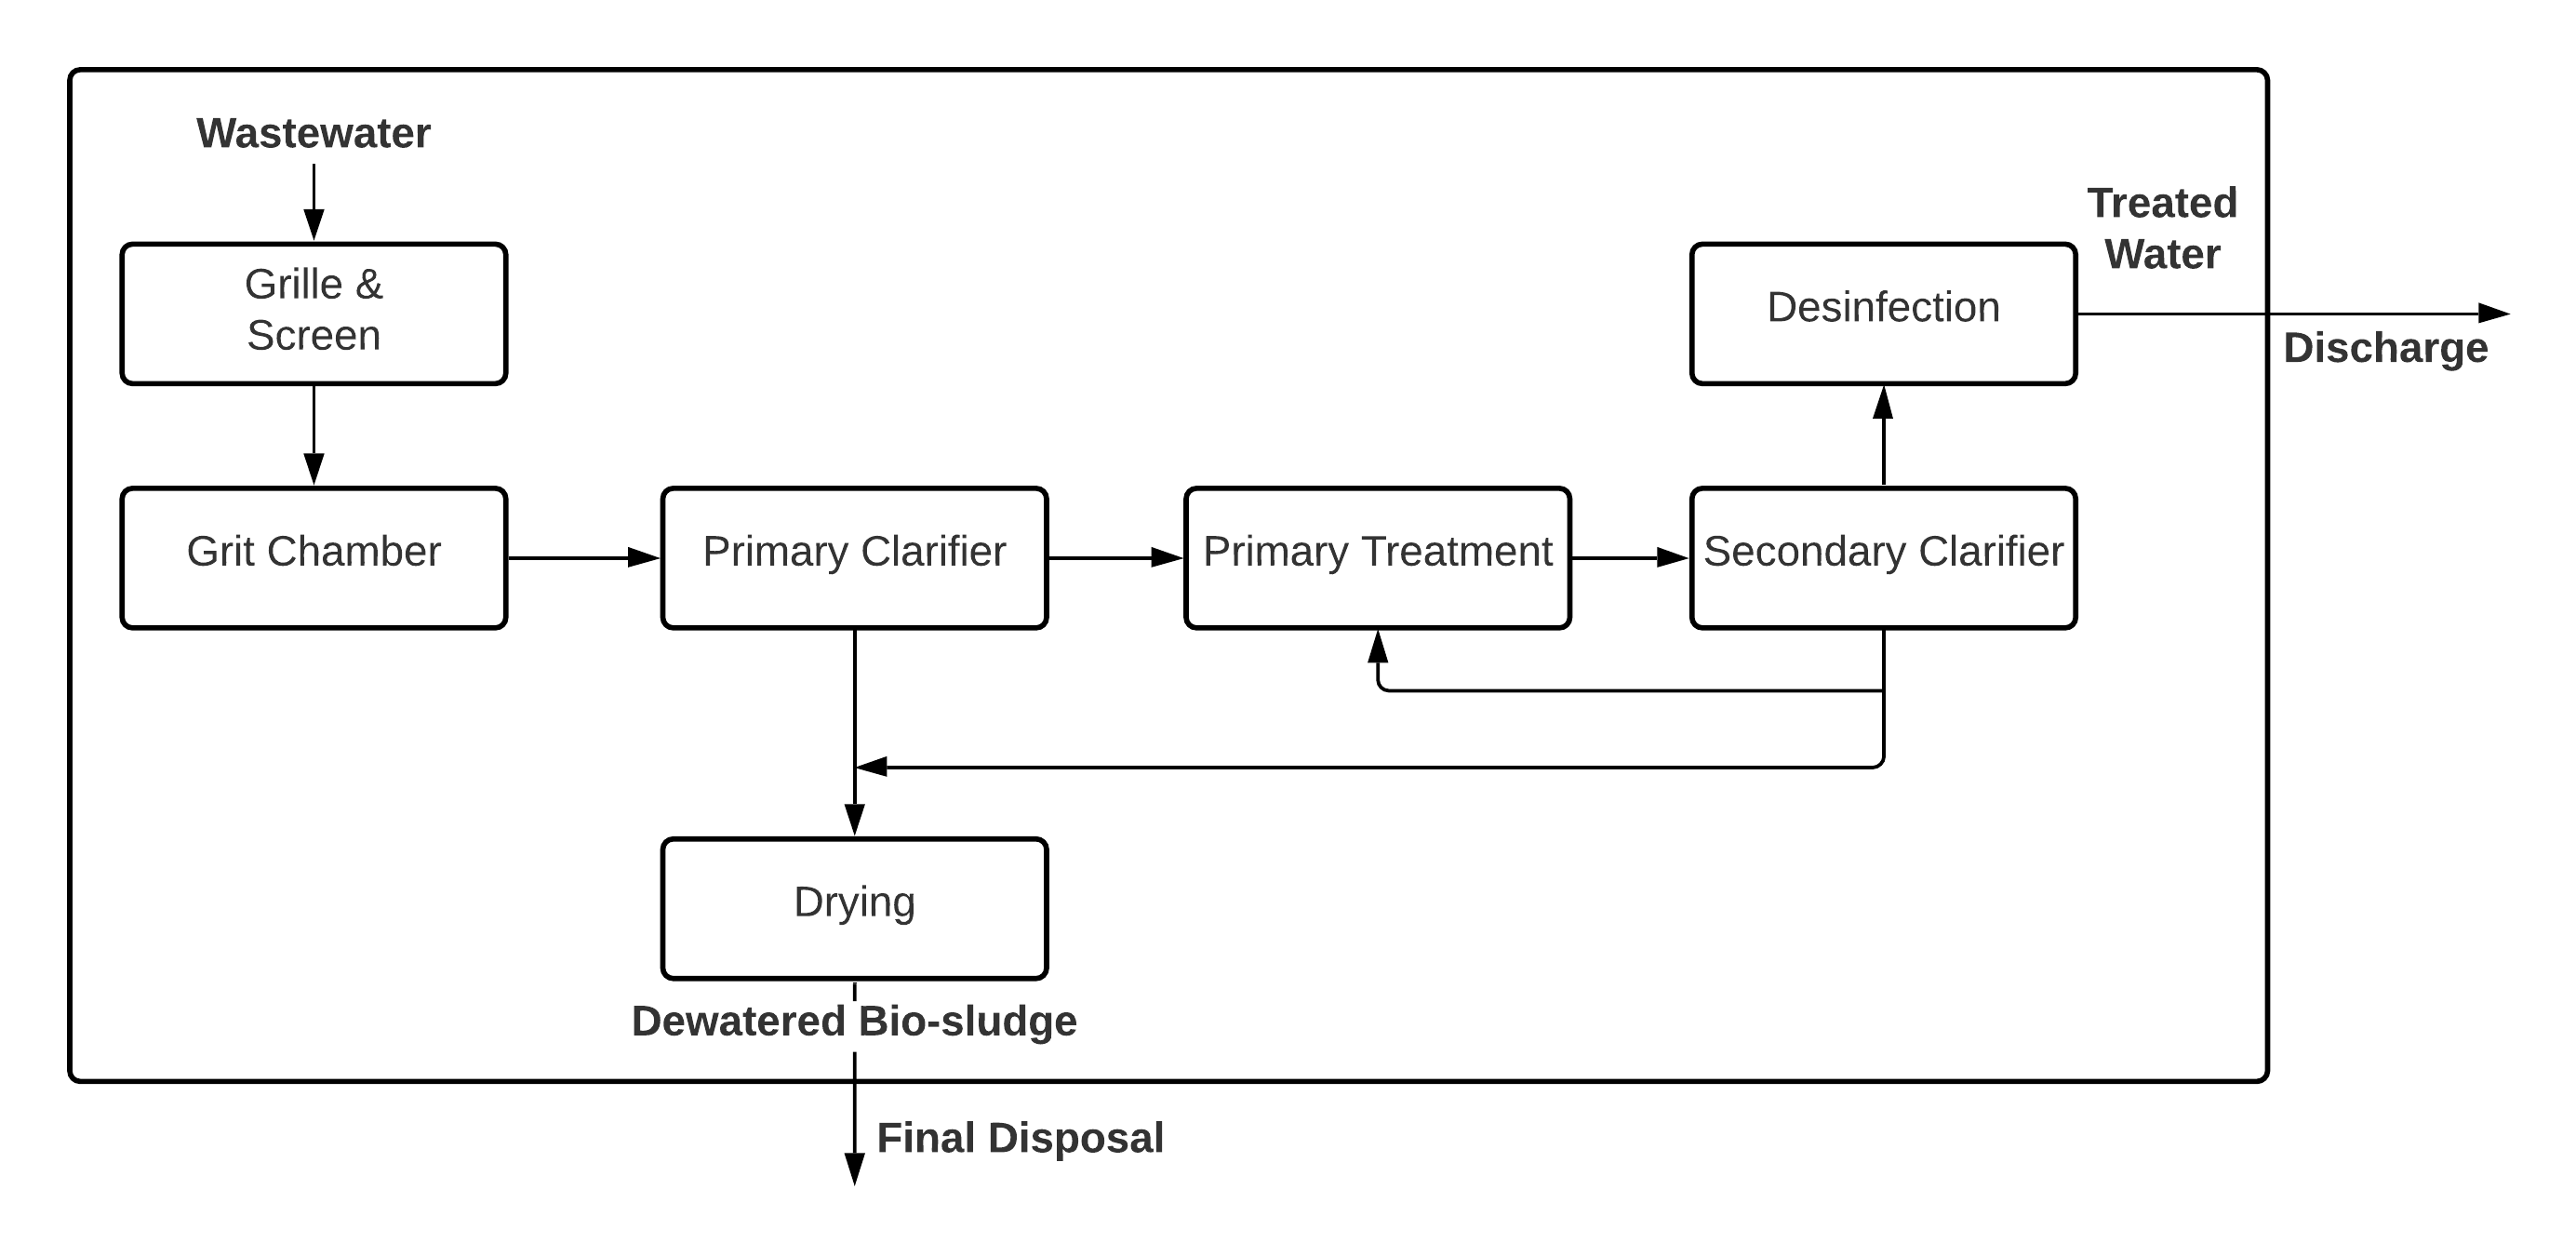
\includegraphics[width=15cm]{figures/Ch2/WWTP.png}
\caption{WWTP Design}
\label{f:wwtp}
\end{figure}

\autoref{f:wwtp} shows the design of a typical \ac{WWTP}, based on the treatment requirements and water contaminants, it results necessary to include some filters, additional settling or equalization tanks.
The \ac{ASP}, a type of Biological treatment, is one of the most used treatments to reduce organic matter (\ac{BOD}, \ac{COD}), nutrients (\ac{TN}, \ac{TP}) and \ac{SS}. In the \ac{ASP}, a microbiological population (mainly protozoa and different types of bacteria) degrade and consume the organic compounds. Most of them require oxygen to live and to commit the task, reason why the bioreactor is usually aerated, providing the right level of \ac{DO} \cite{Haimi2013}. The water flows from the bioreactor to a secondary clarifier which split the clean water and the settled sludge (usually a fraction of the sludge is return to the bioreactor). \autoref{f:ASP} illustrates the \ac{ASP} in a biological stage of a \ac{WWTP}.

\begin{figure}[h]
\centering
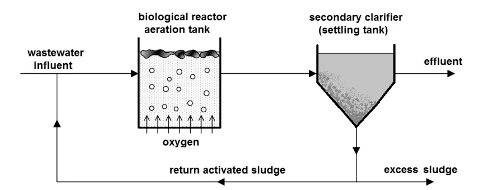
\includegraphics[width=14cm]{figures/Ch2/ASP.png}
\caption{Activated Sludge Process \cite{Fracz2016}}
\label{f:ASP}
\end{figure}

\subsection{Biochemical Oxygen Demand}
The \ac{BOD} is the amount of oxygen required by the microorganisms to break down organic matter for certain period of time (BOD\textsubscript{5}, BOD\textsubscript{10} or BOD\textsubscript{20} where the subscript refers to the number of days, being BOD\textsubscript{5} test the most common one) in a closed container at certain temperature and pH conditions \cite{Wiesmann2007}. \ac{BOD} is used as a measurement of the water quality. The higher level of pollution the higher the amount of organic matter, therefore microorganisms required more oxygen to degrade it.

\subsection{Chemical Oxygen Demand}
The \ac{COD} is the amount of oxygen required to fully oxidize an organic compound in water \cite{Wiesmann2007}. Its measurement requires the use of an oxidant, typically potassium dichromate, to chemically oxidize the organic matter (reaction that consume Oxygen). After the process, the sample is analyzed using an spectrophotometer. Similar to \ac{BOD}, the \ac{COD} works as an indicator of the water quality, an it is very useful in the evaluation of the wastewater treatment efficiency.

\subsection{Volatile Suspended Solids}
In wastewater, there are some settleable solids and non-settleable solids which are suspended in the fluid \cite{Wiesmann2007}. Within the \ac{SS} there is the \ac{MLVSS} which represents the amount of biomass present in the activated sludge. For an efficient pollutants removal process is needed to find a balance between the amount of organic matter (\ac{COD} or \ac{BOD}) and the microorganisms available (\ac{MLVSS}). This relationship is called F/M.

\subsection{Dissolved Oxygen}
\ac{DO} is a relevant factor for the organic matter removal in wastewater treatment process. In the Biological stage must be guaranteed enough \ac{DO} to accomplish the degradation and nitrification of organic matter. Insufficient \ac{DO} level complicates the degradation for the microorganisms. On the other hand, excess of \ac{DO} involves higher energy consumption and lower efficiency in the process \cite{Zhao2021}. 

\section{Machine Learning}
\label{s:Second-Background-Topic}

\ac{ML} is an area of the \ac{AI} where a computer is programmed to learn form data \cite{Ray2019}. In 1959 Arthur Samuel defined the \ac{ML} as \textbf{the field of study that gives the computers the ability to learn without being explicitly programmed}. Almost 40 years later, Tom Mitchell described \ac{ML} as follows: \textbf{A computer program is said to learn from experience E with respect to some task T and some performance measure P, if its performance on T, as measured by P, improves with experience E.} \autoref{f:AI} shows how the \ac{ML} fits in the \ac{AI} world and presents \ac{DL} as part of \ac{ML} which is described in detail in \autoref{s:Second-Background-Deep-Learning}.

\begin{figure}[h]
\centering
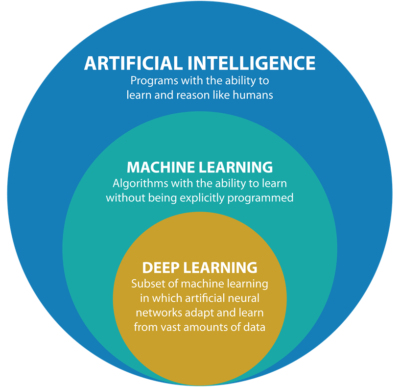
\includegraphics[width=8cm]{figures/Ch2/AI-ML-DL.png}
\caption{AI, ML, and DL \cite{raza_cinquergrana_2018}}
\label{f:AI}
\end{figure}

Now a days machine Learning is used in a variety of fields such as: robotics, biology, social science, virtual personal assistants, computer games, autonomous driving, pattern recognition, natural language processing, computer vision, product recommendation, market prediction, medical diagnosis, fraud detection, agriculture advisory, Bots, climatology, social media services, among others \cite{Srivastava_2019, Shinde_2018, Ray2019}, \autoref{f:Ml-app} shows some of the \ac{ML} application domains. 

\begin{figure}[t]
\centering
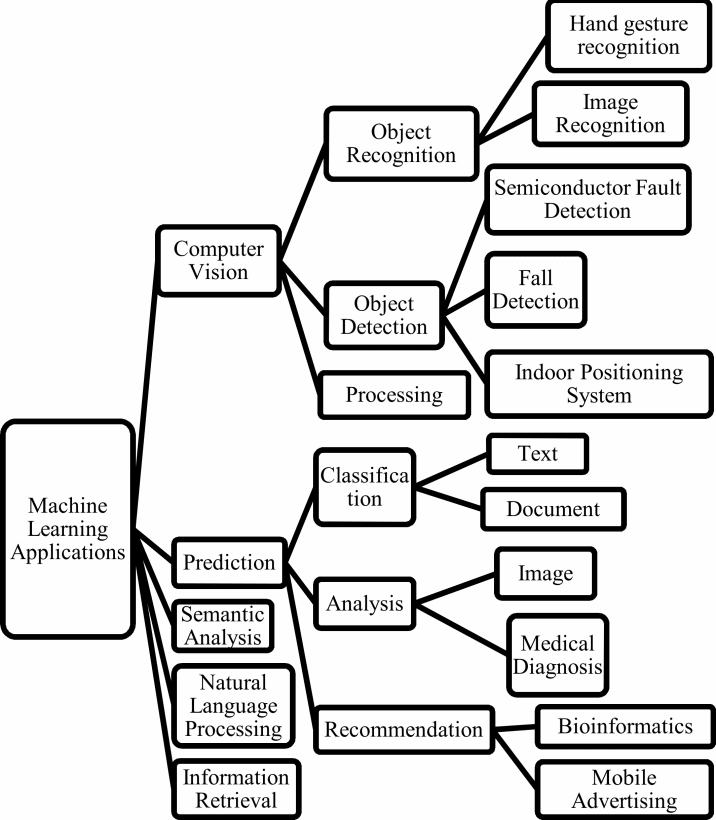
\includegraphics[width=8cm]{figures/Ch2/ML-Applications.png}
\caption{ML Applications \cite{Shinde_2018}}
\label{f:Ml-app}
\end{figure}

\begin{figure}[h]
\centering
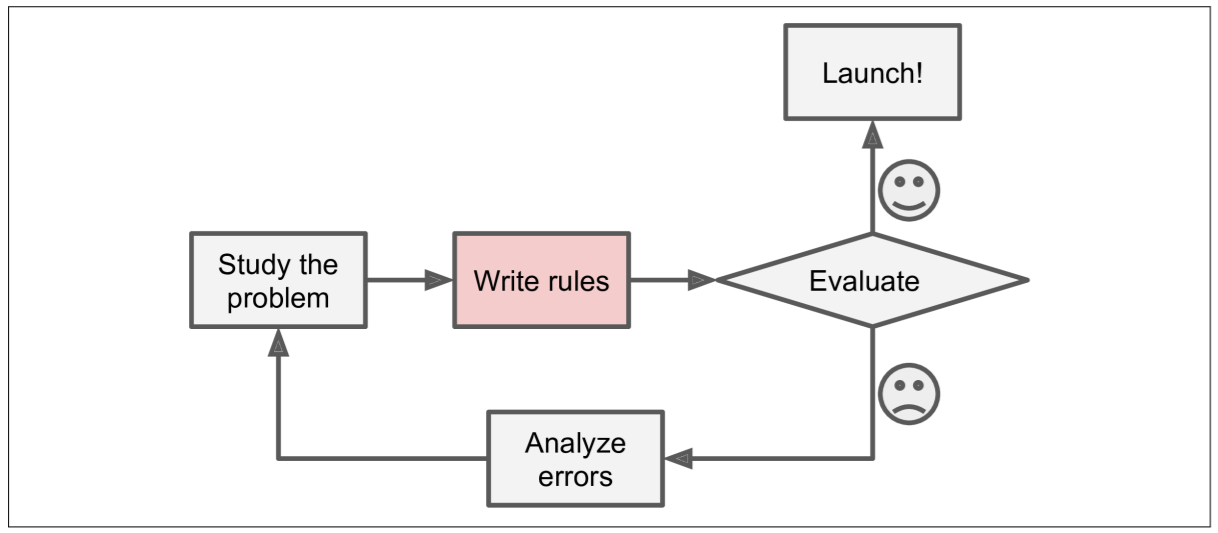
\includegraphics[width=14cm]{figures/Ch2/Tradicional-Approach.png}
\caption{Traditional rule based approach \cite{geron2017}}
\label{f:Traditional-approach}
\end{figure}

An important milestone was the transition from rule based programming to programs that learn automatically based on experience by the use of data. \autoref{f:Traditional-approach} shows how the rule based approach works, it starts by studying the problem, identifying some patterns and building a set of rules based on them. Subsequently, the system is evaluated and the rules are adjusted continuously in an iterative process until a good enough performance is achieved \cite{geron2017}. Should be noted that the bigger the problem the more complex the rules and more difficult the pattern identification task becomes. Meanwhile, \ac{ML} programs improve their performance during the training phase, usually presenting shorter programs, more maintainable, and more accurate. Some studies that compare the results of these data analysis methods evidence that the first tends to provide stronger scientifically sounder information, statistical assessment and uncertainty estimations, but the latter tends to bring forward better accuracy in the majority of works \cite{geron2017,Ye2020}. \autoref{f:ML-approach} illustrates the \ac{ML} approach to solve problems.

\begin{figure}[t]
\centering
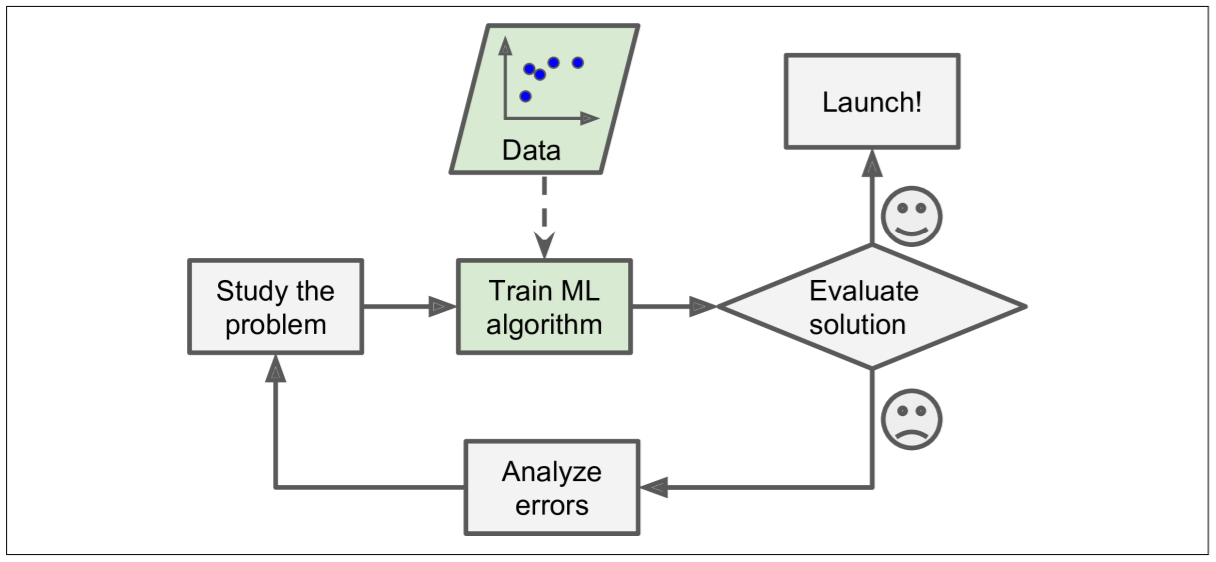
\includegraphics[width=14cm]{figures/Ch2/Ml-Approach.png}
\caption{ML approach \cite{geron2017}}
\label{f:ML-approach}
\end{figure}

\begin{figure}[h]
\centering
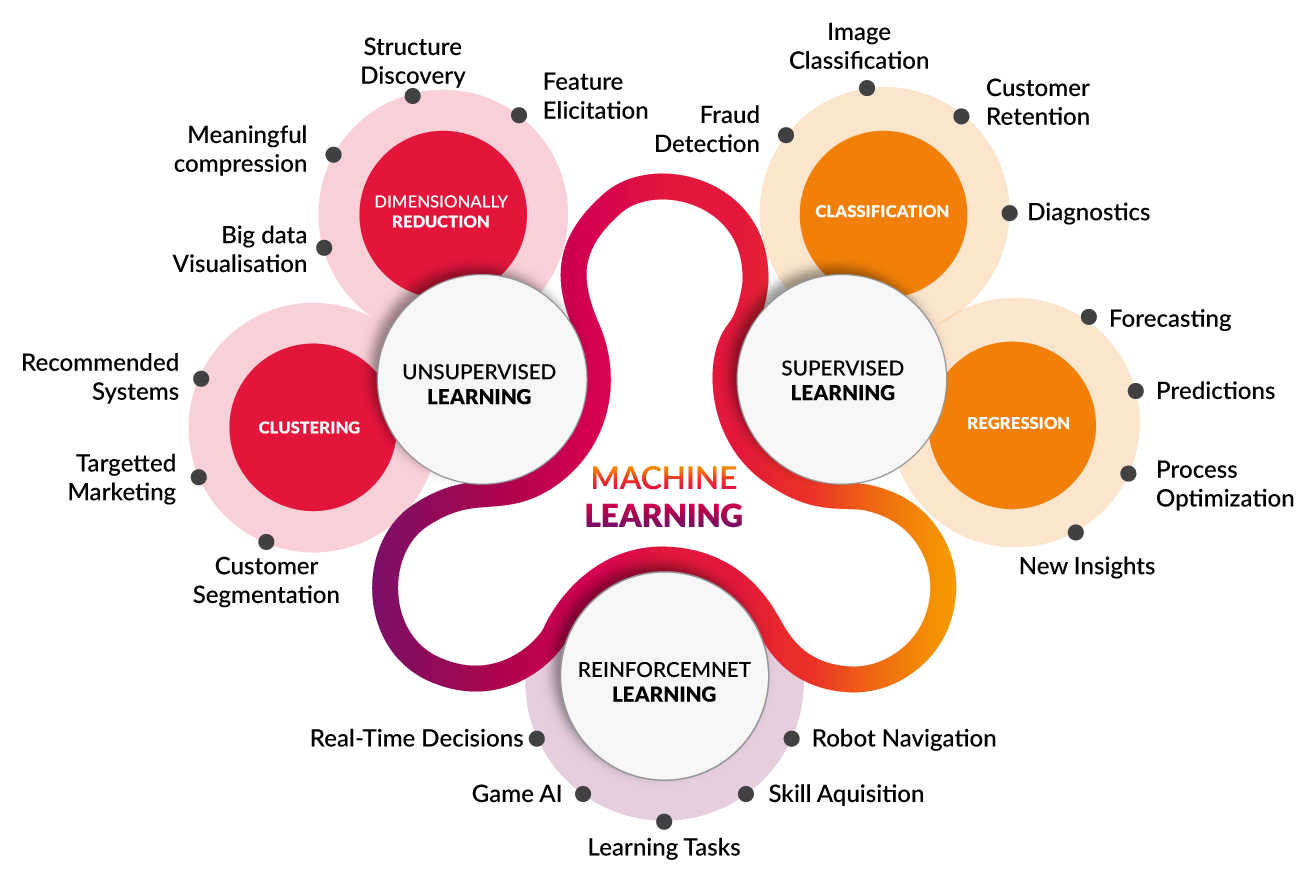
\includegraphics[width=\linewidth]{figures/Ch2/ML-Applications-by-type.png}
\caption{ML applications based on human supervision}
\label{f:ML-App-by-type}
\end{figure}

There are different types of \ac{ML} systems, and they can be classified based on human supervision as supervised learning, unsupervised learning and reinforcement learning. \autoref{f:ML-App-by-type} shows the main tasks of each \ac{ML} type and some of their applications.

\subsection{Supervised Learning}
This category of \ac{ML} algorithms aim to find a function capable of represent the relationship between the input and output variables from a given set of data. It is called supervised since it infers the function from labelled examples during the training stage, which means that for each input sample there is an associated and known output sample assigned by a human supervisor \cite{Batta2020}.

\begin{figure}[h]
\centering
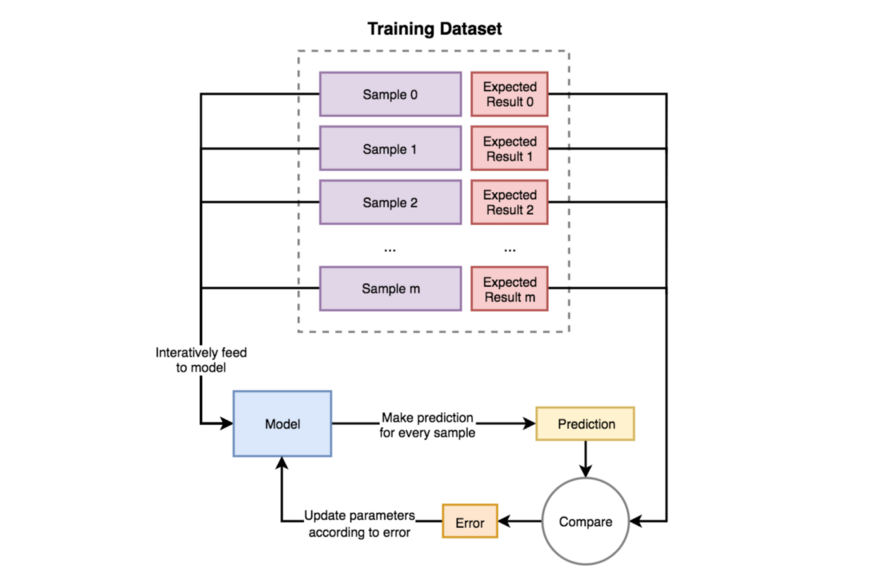
\includegraphics[width=\linewidth]{figures/Ch2/Supervised-Learning.png}
\caption{Supervised Learning}
\label{f:supervised-learning}
\end{figure}

\autoref{f:supervised-learning} present a diagram of how Supervised Learning works\footnote{\url{https://towardsdatascience.com/coding-deep-learning-for-beginners-types-of-machine-learning-b9e651e1ed9d}}. During the training process the model receives the input samples and returns a prediction output for each one using the current parameters values. Each prediction is compared with the expected result, and the difference between them serve as feedback to the model so it can updates the parameters and minimize the error for further iterations.

This type of machine learning is used for both classification and regression problems. Classification is the task of identify the membership of a sample to a category or class, while regression aims to estimate a target numerical value based on the inputs. \autoref{f:classification-regression} presents an example of classification and regression problem. The former uses the information of two genes (input samples) to determine if the subject in study is healthy or suffers a disease, the vertical line depicts the decision boundary of the classification model. The latter, aims to estimate the number of years of the life expectancy for a patient considering some given features. 

\begin{figure}[h]
\centering
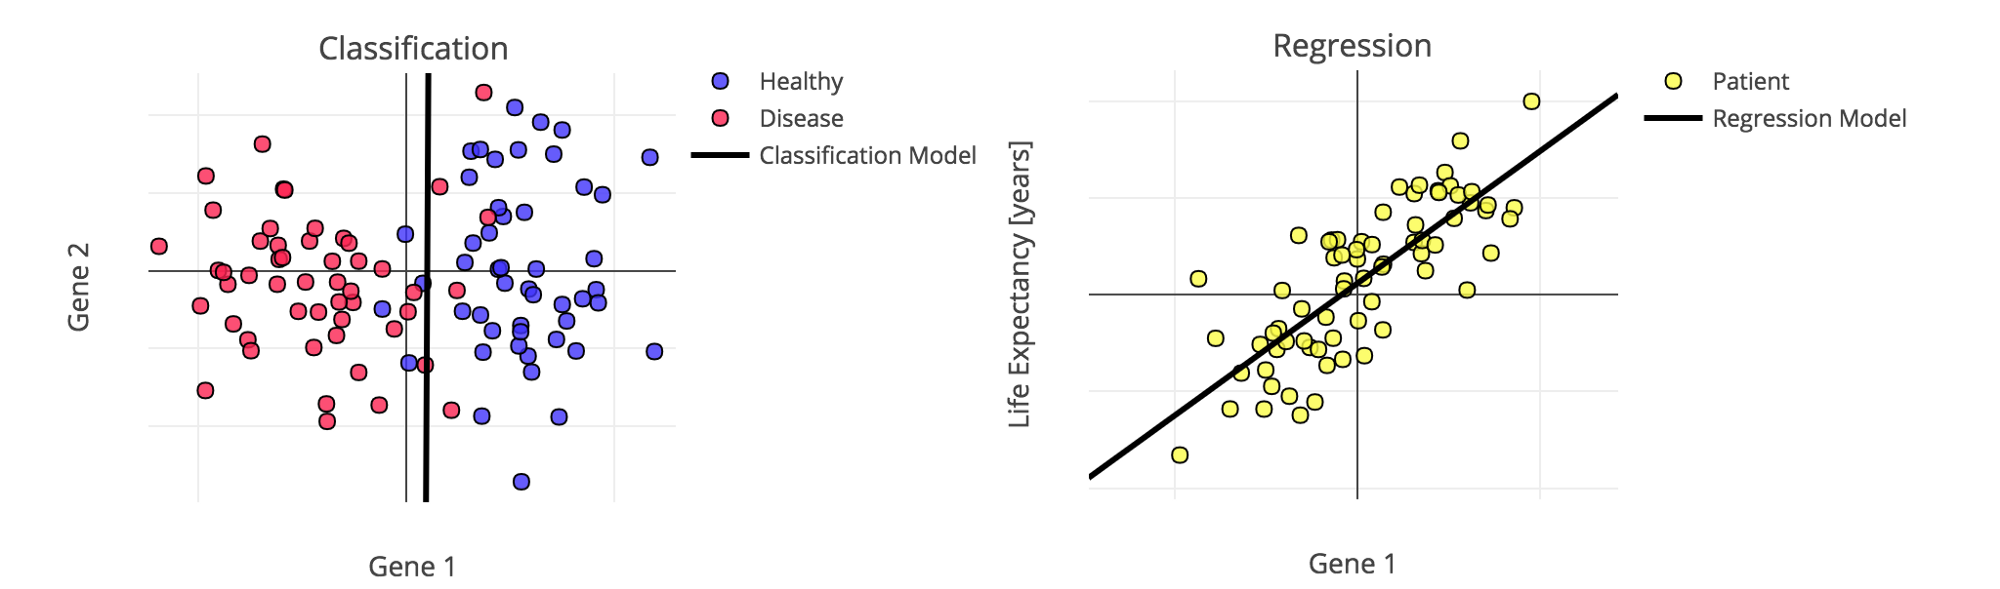
\includegraphics[width=\linewidth]{figures/Ch2/Regression-Classification.png}
\caption{Classification and Regression example}
\label{f:classification-regression}
\end{figure}

\subsubsection{Linear Regression}
A linear model achieves a prediction by calculating a weighted sum of the inputs plus a constant called bias.

\begin{equation}
    \hat{y} = \theta_0 + \theta_1 x_1 + \theta_2 x_2 + ...+ \theta_n x_n\\
\end{equation}

\begin{itemize}
    \item \begin{math}\hat{y}\end{math} is the predicted value.
    \item \begin{math}n\end{math} is the number of features.
    \item \begin{math}x_i\end{math} is the \begin{math}i^{th}\end{math} feature value.
    \item \begin{math}\theta\end{math} is the \begin{math}j^{th}\end{math} model parameter.
\end{itemize}

%\subsubsection{Decision Tree}


\subsubsection{Support Vector Machines}

\ac{SVM} is one of the most powerful and used \ac{ML} technique which stands out for its performance in classification and regression tasks to solve not only linear but non-linear problems too. \ac{SVM} maps the data points from the original space to a higher dimension one. This algorithm looks for an hyperplane capable of achieving the classification or regression of the data in this new space, this dimensionality transformation is also known as the kernel trick\cite{Batta2020}.

\begin{figure}[h]
\centering
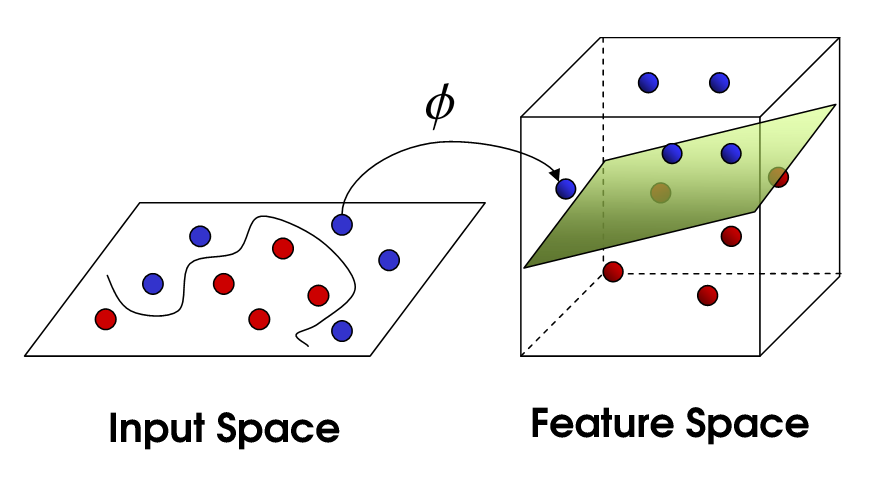
\includegraphics[width=10cm]{figures/Ch2/SVM-KernelTrick.png}
\caption{SVM Kernel Trick}
\label{f:SVM-kernel-trick}
\end{figure}

\autoref{f:SVM-kernel-trick} exemplifies how this works where \begin{math}\phi\end{math} is the function that allows the transformation of the points to the higher dimension space \footnote{\url{https://towardsdatascience.com/the-kernel-trick-c98cdbcaeb3f}}. It is noted that the hyperplane showed works as decision boundary for the classification task presented. \ac{SVM}s fit for complex but small or medium sized datasets \cite{geron2017}.
 
Finally, the problem is reduced to an optimization problem that aims to maximize the minimum distance between the sample points and the hyperplane found which can be observed in \autoref{f:SVM}. \autoref{eq:SVR} presents a equation for the regression version of the \ac{SVM} also called \ac{SVR} \cite{Ye2020}. 

\begin{figure}[h]
\centering
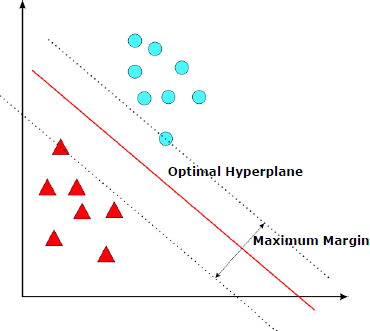
\includegraphics[width=8cm]{figures/Ch2/SVM.png}
\caption{SVM \cite{Hussain2011}}
\label{f:SVM}
\end{figure}

\begin{equation}\label{eq:SVR}
    f(x) = \sum_{i=1}^{M} W_i \phi(x_i) + b
\end{equation}

\begin{itemize}
    \item \begin{math}f(x)\end{math} is the output value.
    \item \begin{math}\phi(x_i)\end{math} denotes space with high-dimensional feature which can be nonlinear.
    \item \begin{math}x_i\end{math} is the \begin{math}i^{th}\end{math} feature value.
    \item \begin{math}W_i\end{math} is the \begin{math}j^{th}\end{math} model parameter.
\end{itemize}

The are several kernels available but the most common ones present in the state-of-the-art are Gaussian Radial Based Function Kernel, Sigmoid Kernel and Polynomial Kernel \cite{Hussain2011}. \autoref{f:SVM-kernels} illustrate this 3 Kernel functions and their equations\footnote{\url{https://www.vebuso.com/2020/03/svm-hyperparameter-tuning-using-gridsearchcv/}}.
\begin{math}\gamma and r \end{math} and d are adjustable kernel functions which are adjusted based on the data.

%\begin{equation}
%    {\textrm{K}}({x_{i}},{x_{j}})=(\gamma {x_{i}}^{\textrm{T}}{x_{j}}+1)^{d}, \gamma >0
%\end{equation}
%\begin{equation}
%    {\textrm{K}}({x_{i}},{x_{j}})=\exp(-\gamma\Vert {x_{i}}-{x_{j}}\Vert^{2}),\ \gamma >0
%\end{equation}
%\begin{equation}
%    {\textrm{K}}({x_{i}}, {x_{j}})=\tanh(\gamma {x_{i}}^{\textrm{T}}{x_{j}}+r)
%\end{equation}

\begin{figure}[h]
\centering
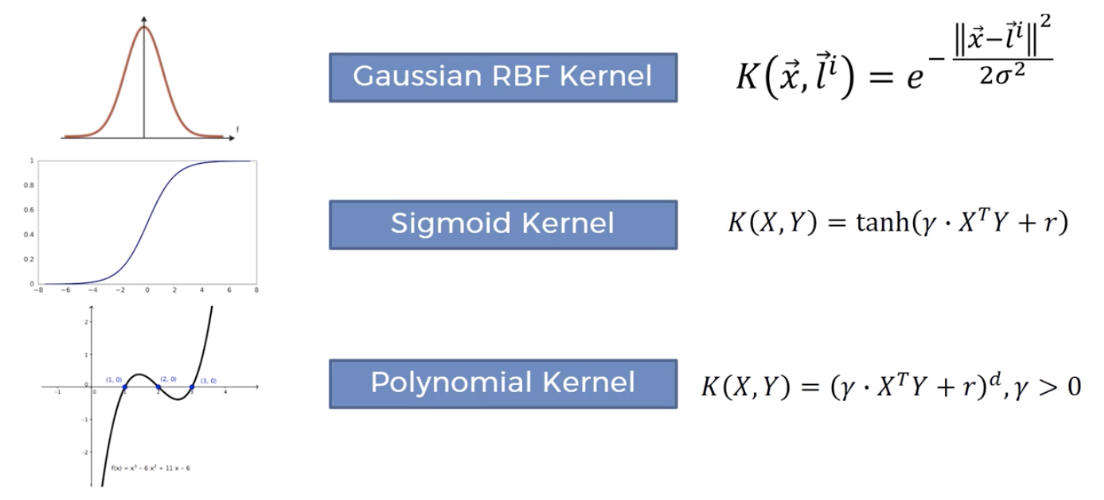
\includegraphics[width=14cm]{figures/Ch2/Kernels.png}
\caption{SVM most used Kernels}
\label{f:SVM-kernels}
\end{figure}

%\subsubsection{Fuzzy Logic}
%\subsubsection{Partial Least Square}

%\subsection{Unsupervised Learning}
%This \ac{ML} category tries to find patterns and make inferences from non-labeled data and it is mainly used for clustering and data dimensionality reduction.  

%\subsubsection{PCA}
%\subsubsection{Clustering}

\section{Deep Learning}
\label{s:Second-Background-Deep-Learning}

\ac{DL} is a subcategory of the \ac{ML} which stands out for its versatility, higher performance, scalability, capacity to face complex and non-linear problems, and the ability of doing feature extraction by itself. \autoref{f:ML-vs-DL} illustrates the capability of \ac{DL} in comparison with \ac{ML}. 

\begin{figure}[h]
\centering
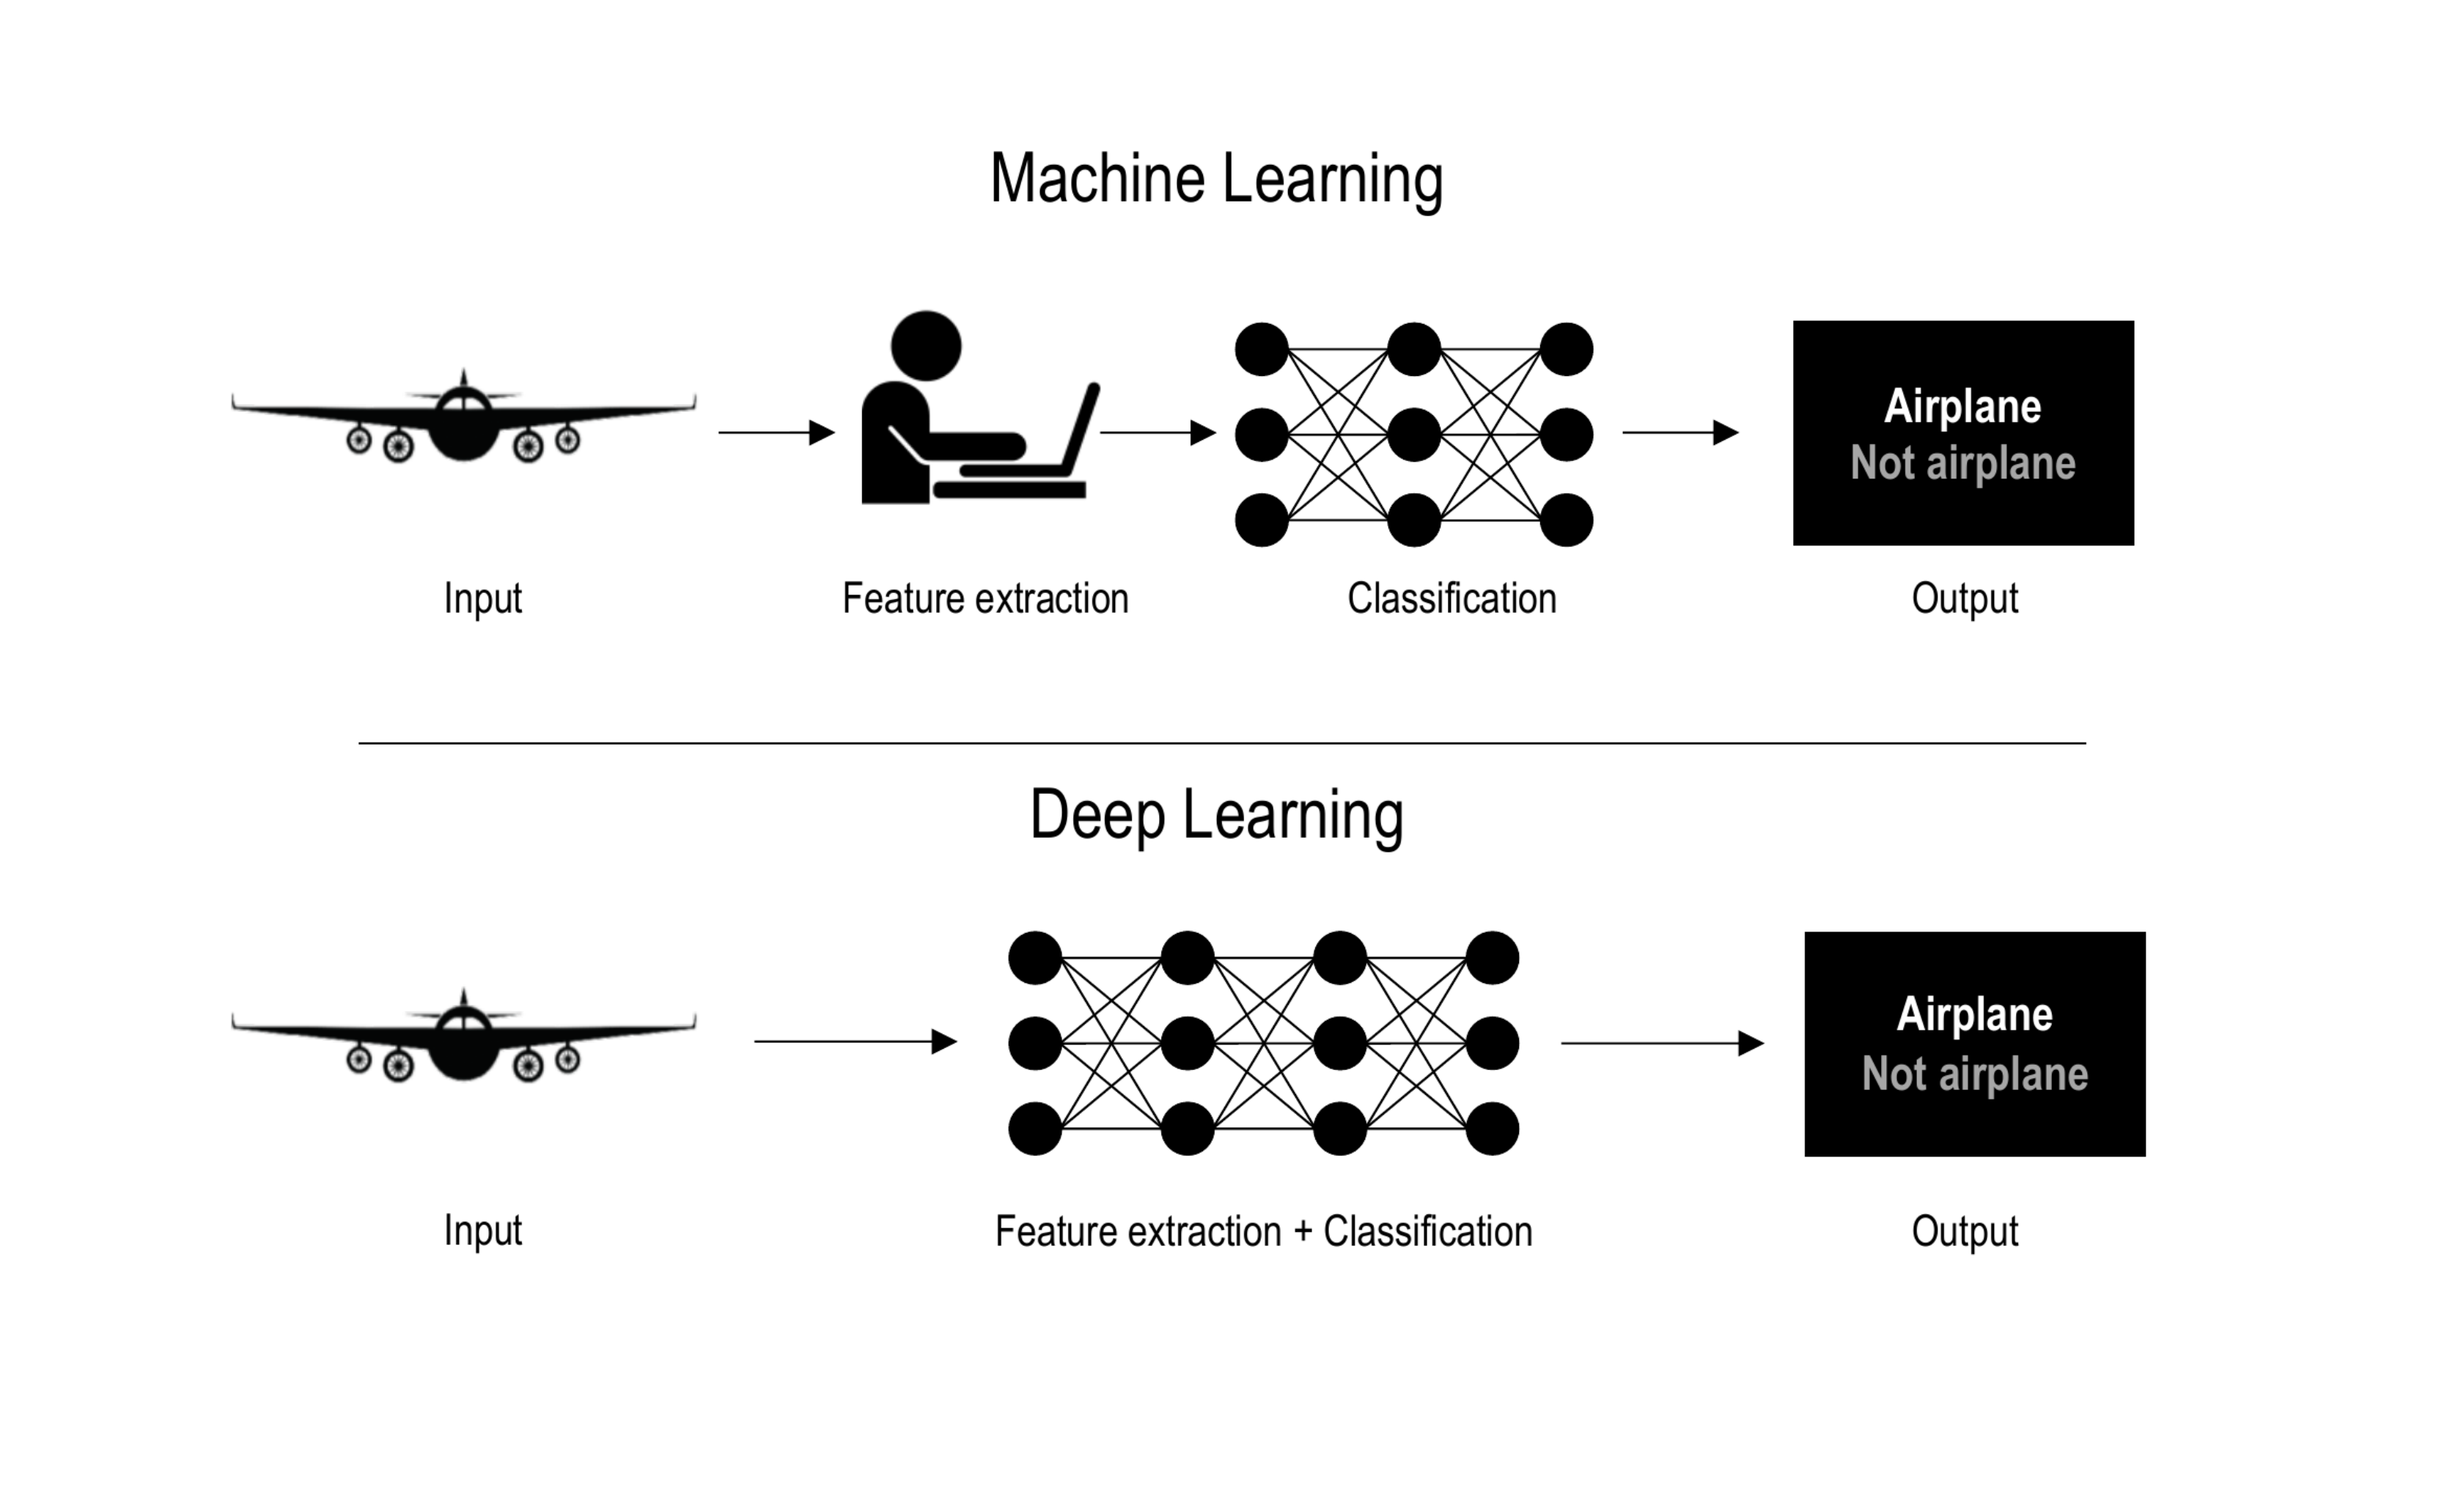
\includegraphics[width=\linewidth]{figures/Ch2/MLvsDL.png}
\caption{ML vs DL}
\label{f:ML-vs-DL}
\end{figure}

Lots of today's inventions are inspired in nature and environment phenomena. Well, the brain architecture has served as inspiration to \ac{ANN} which are the core of the \ac{DL}. An \ac{ANN} model is composed by a set of layers which contains a processing unit called perceptron that emulates a human neuron. Neurons of each layer interconnect with others building a more complex structure with higher learning capabilities just as human brain neuronal connections. This artificial and mathematical connections between perceptrons are called weights. During the training process these weights are updated


\autoref{f:ML-vs-DL-data-amount} shows the scalability and the potential performance based on the amount of data available to train the model.
\begin{figure}[h]
\centering
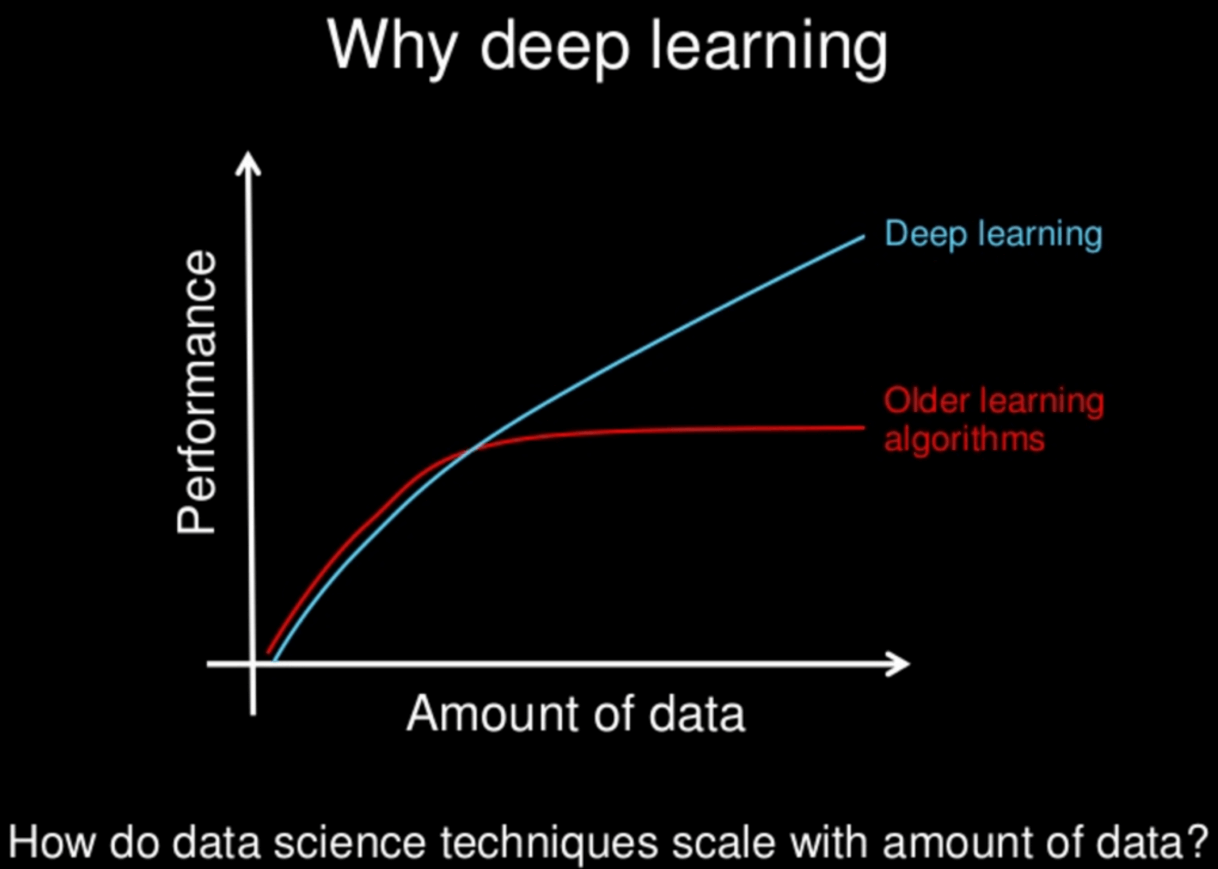
\includegraphics[width=12cm]{figures/Ch2/MlvsDL-data-amount.png}
\caption{ML vs DL performance based on data amount}
\label{f:ML-vs-DL-data-amount}
\end{figure}

\subsubsection{Feed-forward Neural Network}
\subsubsection{Long Short term Memory Neural Network}
In recent years, RNN has shown an outstanding performance in terms of sequential characteristics modelling. As a modified version of RNN, \ac{LSTM} model is specially designed to solve the long-term dependence problem confronted by general RNN methods. LSTM is uniquely added a memory storage module that is protected by some gating neurons who are distinguished from ordinary neurons by setting two states: on and off. Therefore, LSTM is formulated in this research to model sequential characteristics of WTP. Detailed \ac{LSTM} cell model is shown in \autoref{f:LSTM-cell}.

\begin{figure}[h]
\centering
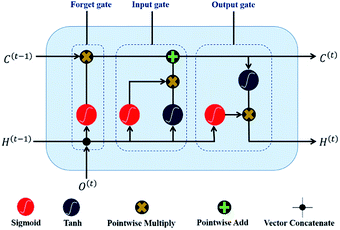
\includegraphics[width=12cm]{figures/Ch2/LSTM_cell.png}
\caption{LSTM cell}
\label{f:LSTM-cell}
\end{figure}

%\subsubsection{Adaptive Neuro-Fuzzy Inference Systems}




\section{Evaluation Metrics}
\label{sec:section_Example}

\subsection{Mean Absolute Percentage Error}

\begin{equation}
    MAPE = 
\end{equation}

%\subsection{Determination Coefficient}

\section{Summary}
\label{s:Background-Summary}

The final section of each chapter should summarize the chapter. In comparison to the chapter.

